\chapter*{$p$-Set \#12}
\addcontentsline{toc}{chapter}{Set \#12}
\markboth{Set \#12}{Set \#12}

\vspace{-0.25in}
\section*{Strassmann Series}

\begin{prob}\label{ex:binom2}\index{Strassmann series!representing $(1+a)^n$}
 Let $p$ be an odd prime and let $a \in p\Z_p$. The identity
\[ \Binom(1+a;n) = (1+a)^{n}\]
proved in Exercise \ref{ex:binomialseries} for nonnegative integers $n$ holds for all $n \in \Z$, since 
\[ (1+a)^{n} = \lim_{m\to\infty} (1+a)^{n+p^m} = \lim_{m\to\infty} \Binom(1+a;n+p^m) = \Binom(1+a;n).\]
\end{prob}

\begin{prob}[Skolem]\label{ex:KC} Let $p$ be an odd prime.  Suppose $a_1, \dots, a_m \in \Z_p$ and $\beta_1, \dots, \beta_m \in 1+p\Z_p$. Let $A \in \Z_p$. There is a Strassmann series $F(T)$ with 
\[ F(n) = a_1 \beta_1^{n} + a_2 \beta_2^{n} + \dots + a_m \beta_m^{n} - A \]
for all integers $n$. Therefore: The equation $a_1 \beta_1^{n} + a_2 \beta_2^{n} + \dots + a_m \beta_m^{n} = A$
is satisfied either for all $n \in \Z$ or for only finitely many integers $n$.
\end{prob}


\section*{An Aside on Cubic Rings}
Exercise \ref{ex:KC} has a lovely application to a cubic analogue of Pell's equation. Before proceeding to that main course, we whet our appetites with some algebraic hors d'oeuvres.\index{$\Z[\sqrt[3]{D}]$, arithmetic of}

% \setlength{\epigraphwidth}{0.56\textwidth}  
% \epigraph{Give first admittance to th' ambassadors.\\
% My news shall be the fruit to that great feast.}{Polonius, \textsl{Hamlet}}
% \setlength{\epigraphwidth}{0.45\textwidth}  

Fix a cubefree integer $D > 1$. Let $\theta$ be the real cube root of $D$ and let $K = \Q(\theta)$. (Thus, $K$ is a subfield of $\R$.) Since $T^3-D \in \Q[T]$ is irreducible over $\Q$ (a cubic polynomial with no roots in the ground field), each element of $K$ has a unique representation in the form $x+y\theta + z\theta^2$ for rational $x, y$, and $z$. 

Fix a complex primitive cube root of $1$, say $\omega$. Then $\theta' := \omega\theta$ and $\theta'' := \omega^2\theta$ are the nonreal complex roots of $T^3-D$. The field $K$ is isomorphic to both $K' = \Q(\theta')$ and $K'' = \Q(\theta'')$ --- indeed, all three fields are isomorphic to $\Q[T]/(T^3-D)$. We will decorate elements of $K$ with $'$ and $''$ to indicate the images in $K'$ and $K''$ under the isomorphisms sending $\theta$ to $\theta'$ and $\theta''$. So $(x+y\theta + z\theta^2)' = x + y\theta' + z\theta'^2$ and similarly for $''$.

For each $\alpha \in K$, the \textsf{norm} $\Nm\alpha$ of $\alpha$ is defined by $\mathrm{N}\alpha= \alpha \alpha' \alpha''$. By a tedious but straightforward calculation,
\begin{equation}\tag{*} \Nm(x+y\theta+z\theta^2) = x^3 + D y^3 + D^2 z^3 - 3Dxyz.\end{equation}
As a consequence, $\Nm\alpha \in \Q$ for all $\alpha \in K$.

Since $'$ and $''$ are isomorphisms, $\Nm(\alpha\beta) = \Nm\alpha \cdot \Nm\beta$ for all $\alpha,\beta \in K$, and $\Nm\alpha \ne 0$ as long as $\alpha \ne 0$. Furthermore, since $\alpha'$ and $\alpha''$ are a complex conjugate pair, $\Nm\alpha = \alpha \alpha' \alpha'' = \alpha |\alpha'|^2$ has the same sign as $\alpha$. 

Our application requires some understanding of the units in the \textsf{pure cubic number ring} $$\Z[\theta] = \{x+y\theta + z\theta^2: x, y, z \in \Z\}.$$ Clearly, $\Z[\theta]^{\times} = \langle -1\rangle \times \Uu$, where $\Uu = \Z[\theta]^{\times} \cap \R^{+}$ is the collection of positive units in $\Z[\theta]$. Proceeding further requires characterizing $\Uu$ norm-theoretically.
%($\Z[\theta]$ is an example of an \textsf{order} in $K$, meaning a subring of the ring of integers of $K$ that contains a $\Q$-basis for $K$.) 

The norm map is integer-valued on $\Z[\theta]$, as one sees from (*). Now if $\varepsilon$ is a positive unit of $\Z[\theta]$, with inverse $\delta \in \Z[\theta]$, then 
\[ 1= \Nm(1) = \Nm(\varepsilon\delta) = \Nm\varepsilon \cdot \Nm\delta. \]
Since $\Nm\varepsilon, \Nm\delta \in \Z^{+}$, it must be that $\Nm\varepsilon= 1$ (and $\Nm\delta = 1$). Conversely, if $\varepsilon = x+y\theta + z\theta^2 \in \Z[\theta]$ with $\Nm\varepsilon=1$, then $\varepsilon > 0$ and
\begin{align*} \varepsilon^{-1} = \varepsilon' \varepsilon'' &= (x+y\theta' + z\theta'^2) (x+y\theta'' + z\theta''^2)
\\ &= x^2 - Dyz + (Dz^2-xy)\theta + (y^2-xz)\theta^2 \in \Z[\theta]. \end{align*}
Hence, $\varepsilon \in \Z[\theta]^{\times} \cap \R^{+} = \Uu$.

Summarizing: $\Uu= \{\varepsilon\in \Z[\theta]: \Nm\varepsilon=1\}$.  

\begin{prob}\label{prob:coeffsisolate} Let $\alpha = x+y\theta+z\theta^2$ with $x,y,z \in \Q$. Then 
\[ 3x = \alpha + \alpha' + \alpha'', \quad 3y \theta = \alpha + \omega^2\alpha' + \omega \alpha'', \quad 3z \theta^2 = \alpha + \omega\alpha' + \omega^2\alpha''. \]
\end{prob}

\begin{prob}\label{prob:discretelattice}For each real number $R > 0$, there are finitely many $\alpha \in \Z[\theta]$ with $|\alpha|, |\alpha'|\le R$. (Here and in Problem \ref{prob:dirichletidea}, $|\cdot|$ is the usual real/complex absolute value.)
\end{prob}

\begin{prob}[Dirichlet's logarithmic embedding]\label{prob:dirichletidea} The map $\Ll\colon \Uu\to \R^2$ defined by $\Ll(\varepsilon) = (\log{\varepsilon},2 \log{|\varepsilon'|})$ is an injective group homomorphism with image $\Ll(\Uu)$ contained in the subspace (line) $\{(x,y)\in \R^2: x+y=0\}$.
% {\scriptsize A nontrivial subgroup of a line through the origin either has all elements equally spaced out (making it cyclic, generated by either of the two points nearest to $\textbf{0}$) or has a cluster point at the origin (meaning that every disc centered at $\textbf{0}$ has an infinite intersection with the group). For $\Ll(\Uu)$, the second case can be ruled out using Problem \ref{prob:discretelattice}. The next exercise asks you to substantiate these claims.}
\end{prob}


\begin{prob}\label{prob:grouplemma} For every additive subgroup $\mathcal{G}$ of $\{(x,y)\in \R^2: x+y=0\}$, one of the following holds:
\begin{enumerate}
\item[(i)] $\mathcal{G} = \{\mathbf{0}\}$,
\item[(ii)] $\mathcal{G}$ is infinite cyclic,
\item[(iii)] some (Euclidean) disc centered at $\mathbf{0}$ has infinite intersection with $\mathcal{G}$.
\end{enumerate}
\end{prob}


{\begin{figure}
\centering
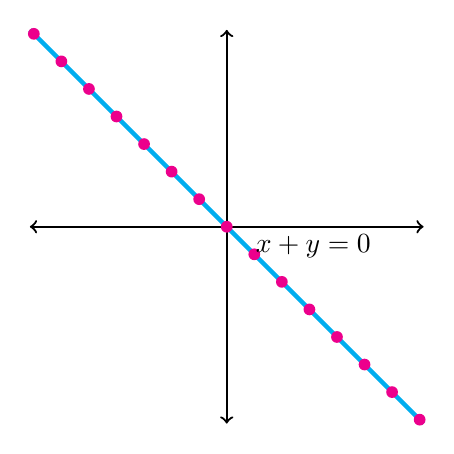
\begin{tikzpicture}[scale=0.5]
\draw[color=cyan, ultra thick] (-5,5) -- (5,-5);
\draw[color=black, thick,->] (0,0) -- (5,0);
\draw[color=black, thick,->] (0,0) -- (-5,0);
\draw[color=black, thick,->] (0,0) -- (0,5);
\draw[color=black, thick,->] (0,0) -- (0,-5);
\node at (0,0) [color=magenta,circle,fill,inner sep=1.5pt]{};
\node at (-0.7,0.7) [color=magenta,circle,fill,inner sep=1.5pt]{};
\node at (-1.4,1.4) [color=magenta,circle,fill,inner sep=1.5pt]{};
\node at (-2.1,2.1) [color=magenta,circle,fill,inner sep=1.5pt]{};
\node at (-2.8,2.8) [color=magenta,circle,fill,inner sep=1.5pt]{};
\node at (-3.5,3.5) [color=magenta,circle,fill,inner sep=1.5pt]{};
\node at (-4.2,4.2) [color=magenta,circle,fill,inner sep=1.5pt]{};
\node at (-4.9,4.9) [color=magenta,circle,fill,inner sep=1.5pt]{};
\node at (0.7,-0.7) [color=magenta,circle,fill,inner sep=1.5pt]{};
\node at (1.4,-1.4) [color=magenta,circle,fill,inner sep=1.5pt]{};
\node at (2.1,-2.1) [color=magenta,circle,fill,inner sep=1.5pt]{};
\node at (2.8,-2.8) [color=magenta,circle,fill,inner sep=1.5pt]{};
\node at (3.5,-3.5) [color=magenta,circle,fill,inner sep=1.5pt]{};
\node at (4.2,-4.2) [color=magenta,circle,fill,inner sep=1.5pt]{};
\node at (4.9,-4.9) [color=magenta,circle,fill,inner sep=1.5pt]{};
\node at (2.2,-0.5) {$x+y=0$};
\end{tikzpicture}
\caption*{Subgroup, shown in pink, of $\{(x,y) \in \R^2: x+y=0\}$}
\end{figure}}
\begin{prob}\label{prob:almostunittheorem} $\Ll(\Uu)= \{\mathbf{0}\}$ or $\Ll(\Uu)$ is infinite cyclic. 
\end{prob}


\setlength{\tabcolsep}{12pt}
\begin{table}[b]
    \begin{minipage}{.5\linewidth}
      \centering
        \begin{tabular}{rr}\toprule
        \multicolumn{1}{r}{$D$} & \multicolumn{1}{r}{$\mu$}\\ \cmidrule(lr){1-1}\cmidrule(lr){2-2} %\morecmidrules \cmidrule(lr){1-1}\cmidrule(lr){2-2}
            2 & $1+\theta+\theta^2$ \\
            3 & $4+3\theta+2\theta^2$ \\
            4 & $5 + 3\theta + 2\theta^2$ \\
            5 & $41 + 24\theta + 14\theta^2$ \\
            6 & $109 + 60\theta + 33 \theta^2$ \\\bottomrule
        \end{tabular}
    \end{minipage}%
    \begin{minipage}{.5\linewidth}
      \centering
        \begin{tabular}{rr}\toprule
            \multicolumn{1}{r}{$D$} & \multicolumn{1}{r}{$\mu$}\\ \cmidrule(lr){1-1}\cmidrule(lr){2-2} %\morecmidrules \cmidrule(lr){1-1}\cmidrule(lr){2-2}
            7 & $4 + 2\theta + \theta^2$ \\
            9 & $4 + 2 \theta + \theta^2$ \\
            10 & $181 + 84 \theta + 39\theta^2$\\
            11 & $89 + 40 \theta + 18\theta^2$ \\
            12 & $9073 + 3963\theta + 1731\theta^2$\\\bottomrule       \end{tabular}
    \end{minipage} 
        \caption*{Generators $\mu$ of $\Uu$ for the first several cubefree $D>1$.}
\end{table}

Since $\Ll$ is an isomorphism from $\Uu$ onto $\Ll(\Uu)$, we conclude from Problem \ref{prob:almostunittheorem} that  $\Uu=\{1\}$ or $\Uu$ is infinite cyclic. With a bit more work, we could show that the second possibility always holds. (Look up the proof of \textsf{Dirichlet's unit theorem} in your favorite algebraic number theory textbook.) For our purposes, having $\Uu =\{1\}$ would only make life easier, so we do not worry about eliminating that (pseudo)possibility.

\section*{A Finiteness Theorem for a Cubic Analogue of Pell's Equation} 
The next two exercises outline a proof of the following theorem.

\begin{thm} Let $D$ be a cubefree integer with $D>1$. Then $x^3-Dy^3=1$ has finitely many integer solutions $x,y$.
\end{thm}

Restricting to cubefree $D> 1$ is not significant: Any $D \in \Z^{+}$ can be factored as $D = D_0 D_1^3$, where $D_0, D_1$ are positive integers with $D_0$ cubefree. Distinct solutions to $x^3-D y^3=1$ give rise to distinct solutions to $x'^3 - D_0 y'^3=1$ (take $x'=x$, $y'=D_1 y$). When $D_0 > 1$, the theorem applies to show that the latter equation has finitely many integer solutions; hence, so does the former. Finally, if $D_0=1$, then $D$ is a cube and each solution to $x^3-Dy^3=1$ yields a way of writing $1$ as a difference of two cubes. But there is only one of these: $1 = 1^3-0^3$. (Why?) So the conclusion of the theorem actually holds for all $D \in \Z^{+}$.

This theorem, first shown by Thue in 1909, stands in sharp contrast with the situation for the classical (quadratic) Pell equation $x^2-Dy^2=1$, which has infinitely many integer solutions for all nonsquare $D\in \Z^{+}$.

We continue with the notation of the last section.  From our work there, \begin{equation}\tag{$\dagger$} x^3-Dy^3=1  \Longleftrightarrow \Nm(x-y\theta)=1\Longleftrightarrow x-y\theta \in \Uu.\end{equation}

If $\Uu=\{1\}$, the equation $x-y\theta\in \Uu$ forces $x=1, y=0$, and we are done proving the theorem already! That was too easy, so we suppose $\Uu = \langle \mu\rangle$, where $\mu$ has infinite order. We may assume that $\mu  > 1$, by replacing $\mu$ with $1/\mu$ if necessary. 

From ($\dagger$), the solutions $x,y \in \Z$ to $x^3-Dy^3= 1$ are in one-to-one correspondence with integers $n$ for which $\mu^n$ has vanishing $\theta^2$-coefficient when written with respect to the basis $1,\theta,\theta^2$. From Problem \ref{prob:coeffsisolate}, if $\mu^n = X + Y\theta + Z\theta^2$, then 
\[ 3Z \theta^2 = \mu^n + \omega \mu'^n + \omega^2 \mu''^n. \]
So we are looking for $n\in \Z$ where $\mu^n + \omega \mu'^n + \omega^2 \mu''^n=0$. This calls to mind Exercise \ref{ex:KC}.

\begin{prob}\label{ex:cubicpell}\label{prob:all1} Let $L = \Q(\theta, \omega)$ ($= \Q(\theta, \theta', \theta'')$). Fix an odd prime $p$ for which $L$ embeds into $\Q_p$. Then $|\theta|_p = |\omega|_p= |\mu|_p = |\mu'|_p =|\mu''|_p = 1$. That is, all of $\theta,\omega, \mu, \mu', \mu''$ belong to $\Z_p^{\times}$.

{\scriptsize Here we abuse notation slightly, using the same symbols for elements of $L$ and corresponding elements of $\Q_p$ under our embedding.}
\end{prob}

\begin{prob}\label{ex:cubicpell2}\label{prob:notconstantzero} Let $L$ and $p$ be as in Exercise \ref{ex:cubicpell}. We would like to apply Exercise \ref{ex:KC} to detect the vanishing of $\mu^n + \omega \mu'^n + \omega^2 \mu''^n$ but there is no reason to expect that $\mu, \mu', \mu'' \in 1 + p\Z_p$. 

To deal with this, set $\nu:= \mu^{p-1}, \nu':= \mu'^{p-1}, \nu'':= \mu''^{p-1}$. These belong to $1+p\Z_p$ by Fermat's little theorem. Writing $n=(p-1)m+r$, 
\[ \mu^n + \omega \mu'^n + \omega^2 \mu''^n= \mu^{r} \nu^m+ \omega \mu'^{r} \nu'^{m} + \omega^2 \mu''^{r} \nu''^{m}. \]
For each fixed $r$, there is some $m \in \Z$ where the right-hand side is nonzero (check this!). Hence, the RHS vanishes for only finitely many $m \in \Z$ (Exercise \ref{ex:KC}). The Theorem follows.\index{cubic Pellian equation}\index{$x^3-Dy^3=1$, finiteness of solutions}\

{\scriptsize Much more is known. For instance, Delaunay and Nagell showed (independently) that $x^3-Dy^3=1$ has at most one integer solution $\ne (1,0)$.}
\end{prob}

\begin{prob}[a striking corollary]\label{prob:strikingcor} Let $\mathcal{P}$ be a finite set of primes and let $\mathcal{D}=\{\prod_{p \in \mathcal{P}} p^{e_p}: \text{each $e_p =0,1,\text{ or }2$}\}$. If $n \in \Z^{+}$ and $n^3+1$ has all prime factors from $\mathcal{P}$, then $(-n)^3-Dy^3=1$ for some integer $y$ and some $D\in \mathcal{D}\setminus\{1\}$.

Deduce: The largest prime factor of $n^3+1$ tends to infinity with $n$.

{\scriptsize By more elaborate methods, Siegel showed that the largest prime factor of $f(n)$ tends to infinity whenever $f(T)\in \Z[T]$ is nonconstant with at least two distinct complex roots.}
\end{prob}


